%%
%% Author: Dario Chinelli & Umberto Zarantonello
%% from 2021-04-15 to 2021-05-28
%%

							% Preamble
\documentclass[11pt]{article}

							% Packages
\usepackage[top=1in, bottom=1in, left=1in, right=1in]{geometry}
\usepackage{amsmath}
\usepackage{enumitem}
\usepackage{amssymb}
\usepackage{tikz}
\usepackage{siunitx}
\usepackage{imakeidx}
\usepackage{graphicx}
\usepackage{subfig}
\graphicspath{ {img/} }
\usepackage{color}   %May be necessary if you want to color links
\usepackage{hyperref}
\hypersetup{
    colorlinks=true, %set true if you want colored links
    linktoc=all,     %set to all if you want both sections and subsections linked
    linkcolor=blue,  %choose some color if you want links to stand out
}
\usepackage{romannum}
							% Document
\begin{document}

\title{\textbf{Appunti del corso di Subatomia} \\
Laurea in Fisica - Università di Ferrara} 

\author{Scritto e impaginato in \LaTeX\ da \textbf{Dario Chinelli} e \textbf{Umberto Zarantonello} nel 2021}

\date{aggiornato al 21 aprile 2021}

\maketitle

\newpage

\tableofcontents

\newpage

							% inizio capitoli
							

% commento

\section{Sezione d'urto}

La \emph{sezione d'urto} è una quantità essenziale che restituisce la misura della probabilità che avvenga una reazione dall'interazione tra due particelle, può essere calcolata solo conoscendo la natura dello "scontro".

Supponiamo di avere un fascio di particelle che interagisce con un bersaglio di spessore $d$, l'area d'interazione è $A$.
Qual è il numero di interazioni al secondo $dN$?
\begin{equation}
\begin{split}
dN &\propto I=\frac{N_i}{At}\\
&\propto \rho A d
\end{split}
\end{equation}
dove $I$ è l'intensità del fascio e corrisponde al numero di particelle incidenti $N_i$ fratto l'area d'incidenza $A$ per il tempo $t$; questa grandezza avrà inoltre una proporzionalità con le caratteristiche del materiale incidente, ciò viene espresso nella seconda formula dove $\rho$ è la densità del materiale incidente, $A$ è sempre l'area d'incidenza e $d$ è lo spessore del campione.
Si ottiene quindi che 
\begin{equation}
\begin{split}
dN &=\frac{KN_i}{At}\cdot\rho Ad\cdot d\Omega\\
dN &=KN_tN_ad\Omega
\end{split}
\end{equation}
il coefficiente $K$ è una grandezza di cui studieremo ora la dimensionalità e sarà proprio ciò che definiremo come \emph{sezione d'urto}.
Nella formula vi sono varie altre grandezze, si ha che:
\begin{itemize}
\item $dN [1/s]$ è il numero di particelle al secondo
\item $N_t=N_i\cdot t [1/s]$ è il numero di particelle incidenti per unità di tempo
\item $N_a=\rho \cdot d[1/m^2]$ è il numero di particelle bersaglio che il fascio colpisce nel cammino.
\end{itemize}
Dall'analisi dimensionale si può vedere che $K$ deve necessariamente avere le dimensioni di un'area, ciò è apparentemente strano in quanto è stato già inizialmente esplicitata all'inizio la natura probabilistica di questa grandezza.
La \emph{sezione d'urto} si definisce quindi come la probabilità che un nucleo del bersaglio interagisca quando il fascio incidente corrisponde ad una particella per unità di area.

Supponiamo ora di considerare un bersaglio sottile soggetto ad un flusso di particelle $F$.
\begin{equation}
F=\biggl[\frac{number}{m^2 s}\biggl]
\end{equation}
Solitamente si fa l'ipotesi di un bersaglio sottile per poter supporre che la particella non subisca più di una collisione e poter così applicare queste formule in modo diretto (nel caso di collisione multiple i calcoli sono più complessi).
La probabilità d'interazione $dP$ è espressa come la sezione d'urto $\sigma$ per il numero di particelle del bersaglio per unità di volume per $dz$
\begin{equation}
dP=\sigma n_b dz
\end{equation}
La variazione del flusso risulterà quindi essere l'inverso del numero totale di particelle incidenti per la probabilità d'interazione (il segno meno tiene conto del fatto che il flusso diminuisce nel tempo, ogni volta che una particella interagisce con il bersaglio viene esclusa dal fascio)
\begin{equation}
\begin{split}
dF&=-FdP=-F\sigma n_b dz\\
\frac{dF}{dz}&=-F\sigma n=-\frac{F}{l}
\end{split}
\label{SD:1}
\end{equation}
Nelle formule ~\eqref{SD:1} abbiamo definito
\begin{equation}
l=1/n\sigma
\end{equation} 
che viene chiamato \emph{libero cammino medio}.
Questa grandezza corrisponde alla lunghezza media che ogni particella percorre senza che subire interazioni.
Alle volte può essere utile ridefinire le grandezze in funzione di $l$ piuttosto che di $\sigma$ perché è una grandezza più visualizzabile e utile sperimentalmente.
Si ottiene quindi quella che è la formula del flusso in funzione di $l$
\begin{equation}
F(z)=F(0)e^{-z/l}
\end{equation}

L'unità di misura delle sezioni d'urto è il barn ($b$). 
Questa unità nasce da delle considerazioni fatte nei primi esperimenti di radioattività.
Dalle considerazioni sui raggi atomici 
\begin{equation}
R=R_0A^{\frac{1}{3}}\hspace{0.5cm} R_0=1,2fm
\end{equation}
Ora, prendendo in considerazione l'uranio $^{239}_{92}U$, in particolare l'isotopo 235, si ottiene un raggio pari a 
\begin{equation}
R[^{235}U]=1,2\cdot (235)^{1/3}=7,4fm
\end{equation}
Che restituisce un'area d'interazione circa
\begin{equation}
\pi R^2(^{235}U)=3\times54\sim 150fm^2
\end{equation}
La misura del barn scelta fu quindi di
\begin{equation}
1barn=100fm^2=100\times 10^{-30}m^2=10^{-28}m^2
\end{equation}
Le sezioni d'urto variano da particella a particella e, mentre per le particelle subatomiche sono relativamente simili, esistono delle particelle particolarmente elusive con sezioni d'urto molto inferiori a quelle classiche.
La sezione d'urto di collisione del neutrino per esempio è estremamente piccola e corrisponde a $10^{-19}mb$ (millibarn).
A causa del valore così basso il neutrino è stato una particella praticamente invisibile per molto tempo e la sua teorizzazione si deve agli esperimenti sul decadimento $\beta$ che davano dei risultati altrimenti anomali.
Un altro esempio è rappresentato dalla materia oscura che è stata rivelata solamente tramite considerazioni gravitazionali ma al giorno d'oggi non vi è ancora nessuna evidenza sperimentale di interazione con la materia in laboratorio.


%%Nuova subsection------------------------------------------------------
\subsection{Esperimento di Rutherford}
Agli inizi del novecento la fisica conosciuta era molto diversa da quella odierna, il fatto che certi materiali potessero emettere delle radiazioni era una conoscenza relativamente recente e questi nuovi effetti sconosciuti avevano evidenziato delle irregolarità nei modelli classici.  
Quando Rutherford fece il suo esperimento erano state già studiate le emissioni $\alpha,\gamma ,\beta$.

L'esperimento di Rutherford fu rivoluzionario per la comprensione della struttura atomica, in quanto rese evidente l'elevata densità di materia del nucleo.
Al tempo infatti il modello atomico ritenuto valido era il \emph{modello a panettone}, che teorizzava un atomo formato da una distribuzione uniforme di carica positiva al cui interno erano presenti degli elettroni che andavano a bilanciare la carica rendendo neutro l'intero sistema.
Le densità di carica positiva e di massa in questo modello dovevano quindi essere basse relativamente a quelle conosciute oggi.
Le grandi intuizioni di Rutherford furono quella di utilizzare il decadimento dei nuclei $\alpha$ come sonda e di adottare un approccio statistico per ovviare al problema di non conoscere la posizione esatta delle particelle.

Per l'emissione alfa furono utilizzati dei nuclei di Radio $^{226}_{88} Ra$.
Il \emph{decadimento} che avviene è il seguente
\begin{equation}
^{226}_{88} Ra \longrightarrow ^{222}_{86}Rn + ^{4}_{2}He + Q
\end{equation}
in questa reazione si conservano il numero di massa totale $ 226 = 222 + 4 $ e la carica totale $ 88 = 86 + 2 $;
$Q$ è il calore emesso dalla reazione esotermica/spontanea, equivalente all'energia data dalla differenza di massa iniziale e finale. 
L'energia cinetica rilasciata nel decadimento che viene trasferita alla particella $\alpha$ è pari a $T = \SI{4.76}{MeV}$.

Lo schema dell'esperimento era piuttosto semplice, un fascio collimato di particelle $\alpha$ veniva indirizzato contro un \emph{target} (lastra sottile di oro) che ampliava il fascio di un certo angolo solido andando a deviare il percorso di una certa porzione di particelle. 
Il fascio uscente veniva quindi rivelato da uno schermo di $ZnS$, mobile su tutto l'angolo solido.
Il fatto sorprendente e inaspettato era che una piccolissima porzione di particelle veniva deflessa ad angoli impossibili per il modello a panettone, erano presenti infatti fenomeni di back scattering ovvero di deviazione di un angolo $\theta=180^o$.
Essenziale fu l'intuizione di Rutherford che non prese tale dato come errore sperimentale ma capì che si trattava di particelle reali.

La sezione d'urto di Rutherford fu calcolata sfruttando semplicemente la meccanica classica. 
Il calcolo si basa sulle leggi di conservazione della meccanica classica e sull'elettromagnetismo. 
Le assunzioni fatte da Rutherford furono:
\begin{itemize}
\item l'interazione deve considerarsi come puramente coulombiana ed elastica;
\item ne il nucleo ne le sonde possiedono spin (anche perché al tempo di Rutherford non era ancora stato scoperto lo spin);
\item il nucleo viene considerato fisso (approssimazione corretta per una differenza notevole di massa).
\end{itemize}

\begin{figure}[h]
\centering
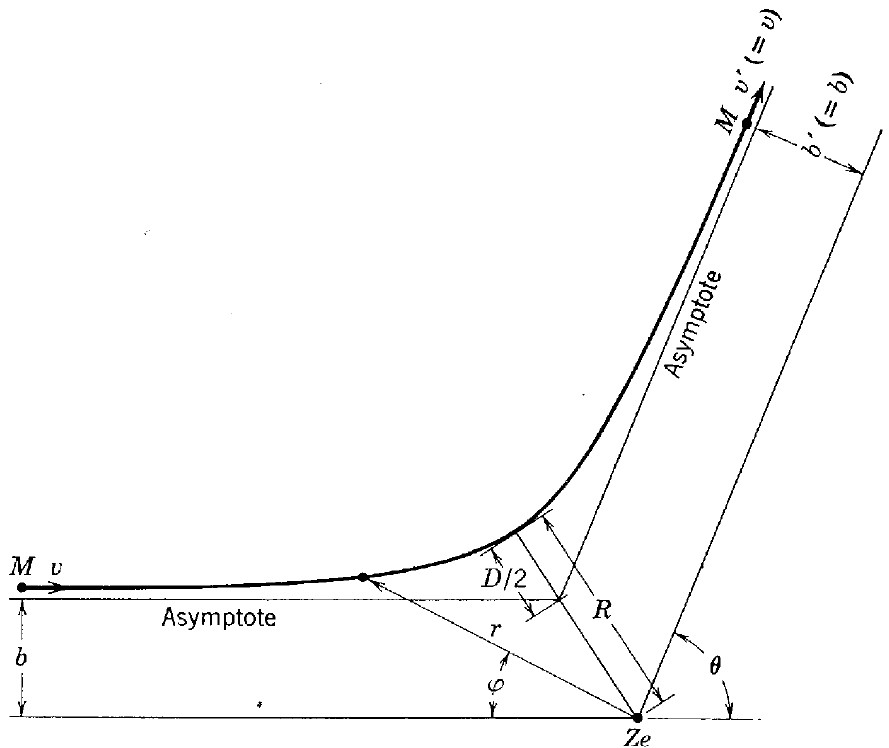
\includegraphics[width=200pt]{fig1_01}
\caption{Traiettoria iperbolica della particella in interazione con un nucleo}
\label{fig:1.1}
\end{figure}
In figura ~\ref{fig:1.1} viene mostrato il modello dello scattering di una particella $\alpha$ di massa M e carica +ze, passante vicino ad un nucleo di carica +Ze.
Il nucleo è fissato al centro del sistema di coordinate.
Prima e dopo la collisione la particella avrà una traiettoria rettilinea (prima con velocità v poi con velocità v') in quanto la forza coulombiana è trascurabile dopo una certa distanza .
Per determinare la posizione della particella si sfruttano le coordinate polari $r(t), \varphi$. 
La distanza tra la traiettoria della particella e la linea parallela passante per il nucleo (asse orizzontale del sistema) è definita come il \emph{parametro d'impatto} $b$.
L'angolo di scattering $\theta$ è dato dall'intersezione dell'asse orizzontale con la parallela alla traiettoria finale passante per il nucleo.

Siccome il nucleo viene considerato fisso, l'energia cinetica finale della particella deve essere identica a quella iniziale. 
Velocità e parametro d'impatto sono costanti prima e dopo l'impatto a causa della conservazione dell'energia cinetica e del momento angolare.
\begin{equation}
Mvb=Mv'b'=L \hspace{1cm} \frac{1}{2}Mv^2=\frac{1}{2}Mv'^2
\end{equation}
\emph{si ha la conservazione del momento angolare perché in presenza di una forza centrale}
\[
dL/dt=\bar r \times \bar F (r)=0
\]
\emph{si ha quindi che raggio e forza sono sempre paralleli}.

Sfruttando nuovamente il momento angolare si cerca ora di ottenere il differenziale del tempo
\begin{equation}
|L|=|\bar r \times m\bar v|=mvb=mv_\perp r=m\omega r^2=m\frac{d\varphi}{dt}r^2
\end{equation}
dove la velocità tangenziale è $v_\perp=\omega r$ e $\omega=d\varphi/dt$ è la velocità angolare. 
Si ottiene quindi
\begin{equation}
\frac{d\varphi}{dt}=\frac{vb}{r^2}\hspace{0.2cm}\to\hspace{0.2cm} dt=d\varphi \frac{r^2}{vb}
\end{equation}
Si può poi introdurre l'interazione elettromagnetica. 
Viene in questo caso sfruttato il teorema dell'impulso
\begin{equation}
\Delta p=\int F_n dt\hspace{1cm}F_n=F\cos\varphi
\end{equation}
dove F è la forza coulombiana tra due particelle
\begin{equation}
F=\frac{1}{4\pi\varepsilon_0}\frac{zZe^2}{r^2}
\end{equation}
La differenza di potenziale risulta essere
\begin{equation}
\Delta p=\int_{-\infty}^{+\infty} \frac{1}{4\pi\varepsilon_0}\frac{zZe^2}{r^2}\cos\varphi dt
\end{equation}
Possiamo quindi sostituire la formula per $dt$ trovata sopra all'interno dell'integrale appena ricavato prestando ovviamente attenzione agli estremi d'integrazione 
\begin{equation}
\begin{split}
t\to -\infty\hspace{2cm}\varphi\to-\frac{1}{2}(\pi-\theta)\\
t\to +\infty\hspace{2cm}\varphi\to+\frac{1}{2}(\pi-\theta)
\end{split}
\end{equation}
\begin{equation}
\Delta p=\int _{-\frac{1}{2}(\pi-\theta)}^{+\frac{1}{2}(\pi-\theta)}\frac{1}{4\pi\varepsilon_0}\frac{zZe^2}{vb}\cos\varphi d\varphi
\end{equation}
Portando fuori dall'integrale tutte le costanti in una constante $A$ si ottiene
\begin{equation}
\Delta p=A[\sin\varphi] _{-\frac{1}{2}(\pi-\theta)}^{+\frac{1}{2}(\pi-\theta)}=A\biggl[\sin\left(\frac{\pi}{2}-\frac{\theta}{2}\right)-\sin\left(\frac{\pi}{2}+\frac{\theta}{2}\right)\biggl]=2A\cos\frac{\theta}{2}
\end{equation}
A questo punto è necessario ricavare la variazione della quantità di moto proiettata sulla normale
\begin{equation}
p_f-p_i=2mv\sin\frac{\theta}{2}
\end{equation}
unendo le due formule per la variazione di quantità di moto si ottiene
\begin{equation}
\begin{split}
2mv\sin\frac{\theta}{2}=2A\cos\frac{\theta}{2} \hspace{0.2cm} & \to \hspace{0.2cm} 2mv\sin\frac{\theta}{2}=\frac{zZe^2}{4\pi \varepsilon_0vb}\cos\frac{\theta}{2}\\
\tan\frac{\theta}{2}=\frac{zZe^2}{4\pi\varepsilon_0mv^2}\frac{1}{b} \hspace{0.2cm} & \to\hspace{0.2cm} \tan\frac{\theta}{2}=K\frac{1}{b}
\end{split}
\end{equation}
$K$ è semplicemente una costante che include tutte le costanti del moto.
Da quest'ultima formula si può vedere che se $b\to 0$ ovvero nel caso di un urto frontale si otterrà come angolo $\theta=\pi$ e quindi la particella sarà rispedita alla sorgente.

\paragraph{Sezione d'urto differenziale}

Si procede ora a ricavare la sezione d'urto differenziale, ovvero lil rapporto differenziale tra le particelle incidenti e quelle scatterate per un certo angolo solido e parametro d'impatto. 
\begin{figure}[h]
\centering
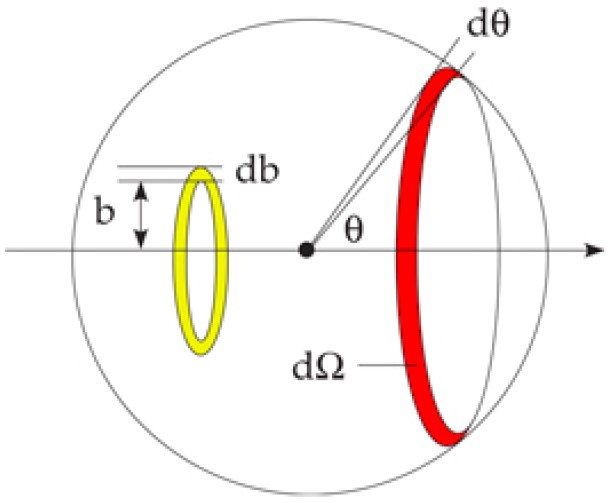
\includegraphics[width=150pt]{fig1_02}
\caption{Schematizzazione della sezione d'urto differenziale in base al parametro d'impatto e all'angolo solido.}
\label{fig:1.2}
\end{figure}

L'area delle particelle incidenti è data dalla formula 
\begin{equation}
d\sigma=2\pi b |db|
\end{equation}
Le particelle definite in quest'area saranno diffuse all'angolo 
\begin{equation}
d\Omega =2\pi \sin\theta d\theta
\end{equation}
Facendo il rapporto tra le due aree si ottiene la sezione d'urto differenziale dal punto di vista cinematico
\begin{equation}
\frac{d\sigma}{d\Omega}=\frac{b(\theta)}{\sin\theta}\frac{db}{d\theta}
\end{equation}

Si può a questo punto unire le formule ricavando $b$ rispetto a $\theta$ 
\begin{equation}
\frac{db}{d\theta}=\frac{d}{d\theta}\biggl|\frac{k}{\tan\frac{\theta}{2}}\biggl|=\frac{K}{\tan^2 \frac{\theta}{2}}\frac{1}{2}\frac{1}{\cos^2\frac{\theta}{2}}
\end{equation}
\begin{equation}
\begin{split}
\frac{d\sigma}{d\Omega}&=\frac{1}{2}\frac{K^2}{\tan^3 \frac{\theta}{2}}\frac{1}{\cos^2\frac{\theta}{2}\sin^2\frac{\theta}{2}}=\frac{K^2}{4\sin^4\frac{\theta}{2}}\\
&=\frac{1}{16}\left(\frac{zZe^2}{4\pi\varepsilon_0 T}\right)\frac{1}{\sin^4\frac{\theta}{2}}
\end{split}
\end{equation}
Introduciamo ora un po' di costanti che aiutano a semplificare questa formula e spesso usate in fisica subatomica
\begin{equation}
\alpha=\frac{b^2}{4\pi\varepsilon_0\hbar c}=\frac{1}{137}\hspace{1cm}\hbar c=197 MeV\cdot fm
\end{equation}
$\alpha$ è denominata \emph{costante di struttura fine}. 

La formula con queste costanti diventa
\begin{equation}
\frac{d\sigma}{d\Omega}=\frac{z^2Z^2}{16}\alpha^2\left(\frac{\hbar c}{T}\right)^2 \frac{1}{\sin^4\frac{\theta}{2}}
\end{equation}
La cosa straordinaria di questa sezione d'urto sta nel fatto che, per delle coincidenze sotto un certo punto di vista fortuite, è uguale a quella calcolata con la meccanica quantistica. Questo succede perché nell'interazione di particelle alfa con il nucleo gli spin sono ininfluenti. 

Commenti alla sezione d'urto:
\begin{itemize}
\item La sezione d'urto diminuisce all'aumentare dell'energia cinetica (inversamente proporzionale a $T^2$).
\item Decresce rapidamente all'aumentare di $\theta$.
\item \'E proporzionale al quadrato delle cariche.
\end{itemize}


%%Nuova subsection--------------------------------------------------
\subsection{Sezione d'Urto Quantistica (Regola d'Oro di Fermi)}
Il cambiamento essenziale che avviene in meccanica quantistica riguarda la probabilità d'interazione. Infatti se nella trattazione classica la probabilità derivava da una serie di considerazioni classiche, nella trattazione quantistica deriva dalla \emph{regola d'oro di Fermi} definita come
\begin{equation}
P=\frac{2\pi}{\hbar}|H_{f,i}|^2\rho(E_f)
\end{equation}
I contributi che compongono questa probabilità d'interazione sono:
\begin{itemize}
\item $H_{f,i}$ è l'elemento dell'Hamiltoniana della perturbazione, ovvero la probabilità che la sezione d'onda iniziale passi alla sezione d'onda finale.
\begin{equation}
H_{f,i}=<f|H|i>=\int \psi*_f(r)H(\bar r)\psi_i d^3r
\end{equation}
(\emph{La probabilità di passaggio di uno stato iniziale ad uno stato finale si valuta effettuando questo integrale tra lo stato iniziale e quello finale della Hamiltoniana di perturbazione}).

Le funzioni d'onda sono quelle che descrivono le nostre particelle $\alpha$
\begin{equation}
H(r)=V(r)=\frac{zZe^2}{4\pi \varepsilon_0r}
\end{equation}
Quali sono quindi gli stati (funzioni d'onda) che descrivono gli alfa?

Ad una certa distanza iniziale saranno onde piane
\begin{equation}
\psi_i \sim e^{ikr} \hspace{1cm}\bar p=\hbar\bar k\hspace{0.5cm}\bar k=\frac{\bar p}{\hbar}
\end{equation}
Dopo l'interazione, ovvero quando le particelle non subiranno più il potenziale coulombiano, si avrà che la funzione sarà nuovamente un'onda piana ma con vettore d'onda variato (legato ovviamente alla quantità di moto)
\begin{equation}
\psi_i \sim e^{ik'r}\hspace{1cm} \bar p'=\hbar\bar k'\hspace{0.5cm}\bar k'=\frac{\bar p'}{\hbar}
\end{equation}
Tornando alla regola d'oro di fermi, ciò mi dice che la probabilità d'interazione dipende dalla probabilità che il mio potenziale faccia passare le mie particelle da una certa quantità di moto ad un'altra.

\item L'altro contributo si ha dalla densità degli stati finali $\rho(E_f)$, ovvero il numero di stati finali accessibili al sistema, maggiore è il tipo di capienza nello spazio delle fasi maggiore è la probabilità. Per ora trascureremo questo contributo per trattarlo più avanti.
\end{itemize}

Studiamo quindi la variabilità della probabilità in base alle funzioni d'onda. 
Si ha
\begin{equation}
H_{f,i}\simeq \int e^{-ik'r} V(r)e^{+ikr}=\int V(r)e^{-i(k'-k)r}
\end{equation}
La variazione dell'impulso in questa trattazione diventa  
\begin{equation}
\begin{split}
\bar p &=\hbar \bar k\\
\bar p &=\hbar k'\\ 
\Delta p =\bar p' -\bar p&=\bar q=\hbar (k'-k)
\end{split}
\end{equation}
Sostituendo nella formula dell'Hamiltoniana si trova
\begin{equation}
\begin{split}
H_{f,i}&=\int V(r) e^{-i\frac{\bar q}{\hbar}r}d^3r\\
&=\frac{zZe^2}{4\pi\varepsilon_0}\int \frac{1}{r}e^{-i\frac{\bar q}{\hbar}r}
\end{split}
\end{equation}
Come si può vedere questa formula corrisponde ad una trasformata di Fourier, e quindi risulta facile risalire alla funzione d'origine. Ciò che si ottiene alla fine è
\begin{equation}
H_{f,i}=\frac{zZe^2}{4\pi\varepsilon_0}\frac{4\pi\hbar^2}{q^2}
\end{equation}
l'ultima frazione è la parte che si utilizza per calcolare la sezione d'urto differenziale
\begin{equation}
\frac{d\sigma}{d\Omega}\propto P\simeq |H_{f,i}|^2\sim\frac{1}{q^4}
\end{equation}
Si può vedere che questa funzione, ricavata quantisticamente, esprime una dipendenza dipendenza proporzionale a $1/q^4$, che corrisponde al momento trasferito ($\delta p$) alla quarta.
 
Sorge spontaneo chiedersi se questo sia consistente con la formula derivata classicamente. La risposta è affermativa e si può dimostrare. Prendiamo infatti la variazione classica della quantità di moto.

\begin{figure}[h]
\centering
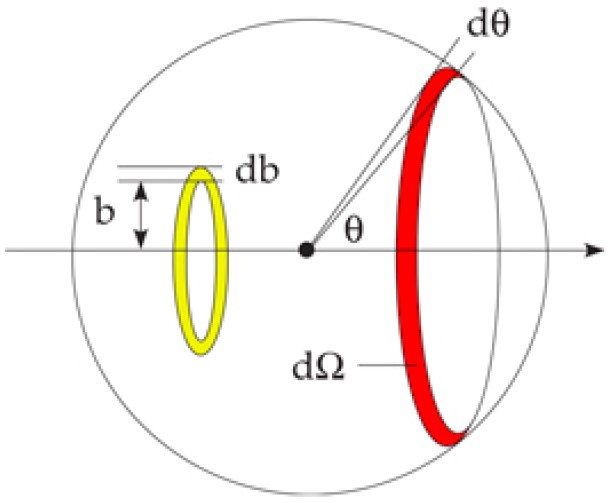
\includegraphics[width=120pt]{fig1_03}
\label{fig:1.3}
\end{figure}

\begin{equation}
\begin{split}
\bar{\Delta p} &=\bar p'-\bar p=q=2p \sin\frac{\theta}{2}\\
q^2 &=4m^2v^2\sin^2 \frac{\theta}{2}
\end{split}
\end{equation}
Ricordando la formula classica dell'energia cinetica
\begin{equation}
T =\frac{1}{2}mv^2
\end{equation}
Si ottiene che 
\begin{equation}
q^2=8mT\sin^2\frac{\theta}{2}
\end{equation}
\'E resa evidente quindi la stessa dipendenza che si aveva nel caso classico, questo è dovuto a vari fattori, ma quello principale è che ci troviamo ad energie non relativistiche.
Altre supposizioni fatte nella trattazione classica erano che le particelle non avessero interazioni di spin, abbiamo trascurato inoltre che i nuclei avessero rinculo. 
Queste sono tutte assunzioni buone ma che per risultati più precisi rilasceremo in trattazioni più avanzate.

\paragraph{Raggio nucleare} Quello che ci si domanda ora è il motivo per cui considerando solamente l'interazione coulombiana si riescano ad ottenere risultati così buoni.

Si consideri il raggio nucleare stimato de Rutherford per la sua trattazione tramite scattering $\alpha$. 
Si cerchi la distanza di massimo avvicinamento della particella a nucleo, che si otterrà per un'energia pari a 
\begin{equation}
V=K_\alpha \hspace{0.5cm}\to \hspace{0.5cm}K_{\alpha}=\frac{1}{4\pi\varepsilon_0}\frac{zZe^2}{R_0}
\end{equation}
Invertendo la formula si ricava il raggio di Rutherford
\begin{equation}
\begin{split}
R_0 &=\frac{1}{4\pi\varepsilon_0}\frac{zZe^2}{K_{\alpha}}\frac{\hbar c}{\hbar c}\\
&\simeq\frac{1}{137}\frac{2\cdot 79}{4\cdot 9 MeV}\hbar c\\
&=46 fm
\end{split}
\end{equation}

Questa è una sovrastima del raggio nucleare in quanto si sa attualmente che il raggio corrisponde ad 8 fermi. 
Questo errore è dovuto al fatto che non vi è interazione nucleare nello scattering di Rutherford ma semplicemente elettrostatica, il che spiega anche la perfetta corrispondenza dei suoi dati con la trattazione teorica.

Supponiamo quindi di riuscire ad aumentare l'energia delle particelle $\alpha$ (quello che accade negli acceleratori). 
Si supponga poi di utilizzare come target del piombo e di porre un rivelatore a $60^o$. 
\begin{figure}[h]
\centering
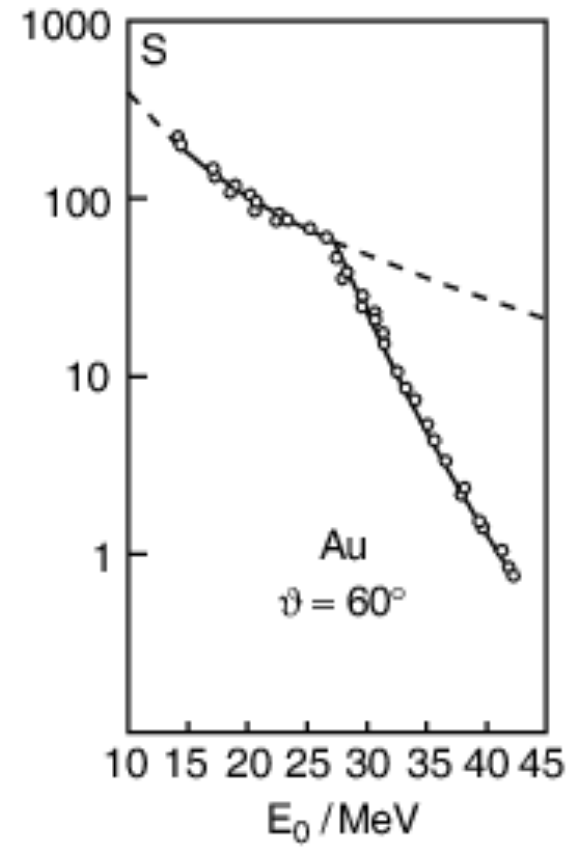
\includegraphics[width=120pt]{fig1_05}
\caption{Esperimento di Rutherford su target di piombo in confronto al risultato calassico}
\end{figure}
Si può osservare che l'andamento del numero di particelle scatterate per energie inferiori a 27,5 MeV rispecchia esattamente l'andamento di Rutherford ma poi ha un cambio drastico. 
Questo accade perché oltre un certo raggio subentra l'interazione per forza forte
\begin{equation}
R=\frac{Q_1Q_2}{4\pi\varepsilon_0KE}=8.59 fm
\end{equation}
La sovrastima di Rutherford era dovuta al fatto che le particelle da lui usate avevano effettivamente interazione puramente coulombiana.


%%Nuova subsection-----------------------------------------------------
\subsection{Derivazione con l'Elettrodinamica Quantistica}
Questa trattazione è possibile in modo semplice grazie ai diagrammi di Feynman che semplificano il tecnicismo della fisica teorica rendendola accessibile ai fisici sperimentali.
\begin{figure}[h]
\centering
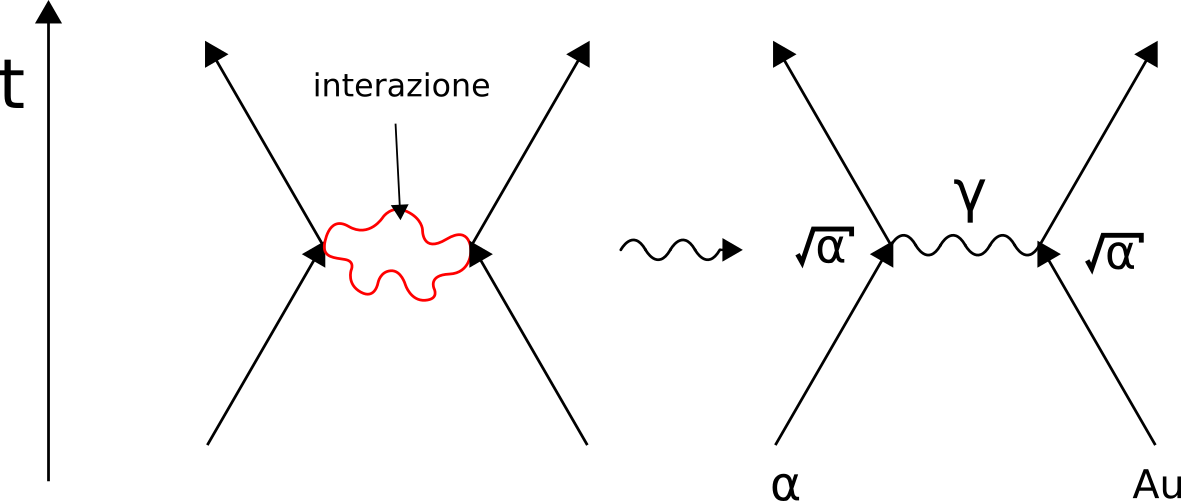
\includegraphics[width=300pt]{fig1_04}
\caption{Diagrammmi di Feynman}
\end{figure}
Secondo i diagrammi di Feynman ogni particella reale è descritta da una linea continua. Una cosa da tenere sempre presente è la direzione in cui si svolge l'azione temporale, in questo caso si svolge verso l'alto ma è solamente una rappresentazione grafica di un'interazione.
Nelle teorie quantistiche di campo l'interazione viene descritta tramite lo scambio di una particella.
La grande novità che è stata introdotta da queste teorie è che l'interazione non sia descritta tramite un campo ma attraverso lo scambio di particelle virtuali.

Come si ricava quindi la sezione d'urto?

La particella alfa emette un fotone virtuale e questo viene descritto tramite una costante di accoppiamento posta ai vertici (ovvero nel punto d'impatto) denominata $\sqrt{\alpha}$. 
L'interazione viene rappresentata da quello che si chiama propagatore ovvero la linea interna che congiunge i due vertici.
\begin{equation}
\propto \frac{1}{Q^2+M^2C^2}
\end{equation}
dove $Q^2$ è il momento trasferito, $M$ è la massa della particella mediatrice (bosone vettore), $\gamma$ è il fotone.
Come si calcola l'ampiezza della transizione?
\begin{equation}
\begin{split}
|M_{f,i}| &=\sqrt{\alpha}\frac{1}{Q^2}\sqrt{\alpha}=\frac{\alpha}{Q^2}\\
P &\propto |M_{f,i}|^2 =\frac{\alpha^2}{Q^4}
\end{split}
\end{equation}
Dove P è la probabilità di transizione della particella, corrispondente alla sezione d'urto.
Si può notare anche qui che la proporzionalità trovata per le altre trattazione è mantenuta.




%Zarantonello Umberto 20/04/21

\section{Il Nucleo}
La secoda particella ad essere rivelata dopo l'elettrone fu il protone. 
La prima evidenza sperimentale è dovuta a Rutherford nel 1917 sfruttando sempre le particelle alfa, questa volta in collisione con l'aria dove è presente l'azoto N 
\begin{equation}
^4_2He +^{14}_{7}N_{7}\longrightarrow ^{17}_8O_9+protone
\end{equation}
Al tempo uno dei modelli nucleari era che il nucleo fosse composto da un certo numero $A$ di protoni ed un numero $A-Z$ di elettroni (con Z il numero di elettroni della nuvola elettronica) in modo da bilanciare la carica dei protoni rendendo l'atomo stabile.
Analizziamo dunque la possibilità di avere un nucleo di questo tipo.
Che potenziale elettroagnetico dovrebbero gestire i protoni?
\[E=\frac{Ze^2}{4\pi\varepsilon_0R}\]
dove $R=R_0 A^{1/3}=1.2fm\cdot A^{1/3}$ (formula empirica per il calcolo del raggio nucleare). 
Calcolando si ottiene quindi
\[E=-1.20\frac{Z}{A^{1/3}MeV}\]
Per esempio, ponendo A=140 e Z=58 l'energia cinetica che si ottiene è $E=-13.4MeV$ (elettrone con energia relativistica quindi $E=pc$). Un elettrone con tale energia cinetica è possibile che resti confinato all'interno del nucleo?
\[\lambda=\frac{h}{p}=2\pi \frac{\hbar c}{pc}=\frac{2\cdot 3.14\cdot 200MeV\cdot fm}{13.4MeV}\simeq 90fm\]
L'elettrone non può essere quindi confinato nel nucleo perchè la sua lunghezza d'onda è molto maggiore.

\paragraph{La scoperta del Neutrone} fu fatta da Chadwick che fu il primo ad intuire, da un'esperienza che in realtà era già stata fatta da più fisici, la presenza di un'altra particella. 
La situazione che si verificava era che tramite l'emissione di particelle alfa generate dal polonio, fatte collidere su un target di Berilio, si otteneva una radiazione che riusciva ad attraversare uno schermo spesso di piombo, il che suggeriva il fatto che fosse una radiazione neutra (impossibile per della radiazione carica attraversare uno schermo troppo spesso). 
Al tempo l'unica radiazione neutra conosciuta era la radiazione elettromagnetica il che fece pensare ad una reazione cle tipo
\[
^9_4Be+^4_2He\longrightarrow[^{13}_6C*]\longrightarrow^{13}_6C+\gamma
\]
Con uno stato intermedio dato da uno stato eccitato del carbonio 13.
Un ulteriore passaggio fu quello di aggiungere dopo lo schermo di Piombo $Pb$ una lastra di paraffina da cui, dopo l'interazione con la radiazione, emergevano protoni con energia pari a $E=7,5MeV$. 
La radiazione gamma doveva quindi possedere un'energia in grado di podurre dei protoni di energia 7,5MeV trammite scattering Compton il che riconduce ad un'energia minima di 55MeV.
Quando il Berilio assorbiva le particelle alfa quest'ultime si trovavano ad un energia di 5MeV, essendo poi una reazione esotermica si aveva che il Q della reazione corrispondeva a $Q=10MeV$, il che riconduceva ad un energia massima disponibile di 14MeV.
L'unica spiegazione possibile era che si trattava quindi di una particella nuova, neutra e con la stessa massa del protone.


%Zarantonello Umberto 22/04/21
\section{Esercizi}
\subsection{Settimana 1}
\paragraph{Es. 1:}
Si calcoli la velocità media di:
\begin{itemize}
\item Molecole d'aria a temperatura ambiente
\item Eletroni atomo idrogeno
\item Terra attorno al sole
\item Elettroni che escono da un vecchio tubo catodico
\end{itemize}
\paragraph{Ris.:}
\begin{itemize}
\item \textbf{Molceole d'aria}
supponiamo di essere a $20^oC$ corrispondenti a $293K$ si sfrutti la teoria cinetica dei gas
\begin{equation}
\frac{3}{2}K_BT=\frac{1}{2}m<v^2>
\end{equation}
Si approssimi l'aria come azoto $N_2$ la cui massa molecolare è $M_{N_2}=28$
si ottiene
\[
\sqrt{<v^2>}=\sqrt{\frac{3K_BT}{m_{N_2}}}=\sqrt{\frac{3\times1,3\times10^{-23}293}{28\cdot 1,66\times10^{-27}kg}}=510\frac{m}{s}
\]
\item \textbf{Elettroni dell'idrogeno}
Ricordando la costante di Ridberg ovvero il potenziale di dissociazione dell'idrogeno, questa può essere considerata pari alla sua energia cinetica.
\[
E=13.5eV=K_e\\
K=135\times10\cdot1,6\times10^{-19}J=2,1\times10^{-18}J=\frac{1}{2}m_ev^2
\]
conoscendo la massa dell'elettrone corrispondente a $m_e=9,1\times10^{-31}kg$ si ottiene che la velocità dell'elettrone sarà
\[
v_e=\sqrt{\frac{2K_e}{m_e}}=2,1\times10^6\frac{m}{s}
\]
Si può notare che questa è una conferma che l'elettrone sia una particella non relativistica.
\end{itemize}
Si lasciano al lettore gli altri due punti.

\paragraph{Es. 2:}
Si calcoli il numero di molecole nell'atmosfera.
\paragraph{Ris.:}
Si parte considerando la massa dell'atmosfera, che si può calcolare partendo dalla pressione atmosferica, corrispondente al dell'aria sopra un metro quadro.
\[
p=10^5\frac{N}{m^2}\longrightarrow M=10^4\frac{kg}{m^2}
\]
Si consideri, ora la superficie della terra 
\[
A_{terra}=4\pi R^2=12(6\times10^6m)^4=4\times10^14m^2
\]
Si può quindi trovare la massa dell'aria
\[
M_{aria}=10^4\frac{kg}{m^2}4\times10^{14}m^2=4\times10^{18}kg
\]
Per calcolare il numero di molecoe di aria, si consideri il pero molecolare di azoto e ossigeno
\[
N_2=28\hspace{0,5cm}O_2=32
\]
Il che in media corrisponde ad un peso molecolare di $30$.
Una mole peserà dunque $30g$
\[
M_{aria}=\frac{4\times10^21g}{30g/mol}=1,3\times10^{20}mol
\]
Il numero di molecole d'aria corrispondera quindi alla massa in moli dell'aria moltiplicata per il numero di Avogadro $N_A=6\times10^{23}$
\[
N_{aria}=M_{aria}\times N_A\simeq 10^41molecole
\]
Se si volesse poi sapere quante molecole di aria dell'ultimo respiro di Carlo Magno sono contenute nei nostri polmoni, si dovrebbe fare il rapporto fra la quantità di aria contenuta nei nostri polmoni e quella contenuta nell'atmosfera.
\[
1mole (STP)=20L
\]
Una mole in condizioni standard corrisponde a 20 litri, la densità dell'aria corrisponderà quindi a 
\[
30\frac{g}{mol}:20\frac{L}{mol}=1,5\frac{g}{L}\\
1L\sim 1g\sim 3\times 10^{22}molecole
\]
Qual è la frazione di molecole che noi respiriamo ad ogni respiro?
La massa dell'aria totale è pari a $4\times 10^21g$ e ogni respiro corrsponde ad un peso di circa $1g$, il che restituisce un rapporto di
\[
0,25\times 10^{-21}
\]

\paragraph{Es. 3:}
si calcoli l'energia contenuta in un $kg$ di benzina, pprossimando la benzina come $CH_2$.
\paragraph{Ris.:}
Si può stimare che per ogni legame chimico l'energia sia pari a $E=1,5eV$ (\'E una stima molto approssimata).
Si considerino le masse atomiche:

Il carbonio ha massa atomica $C=12$, mentre l'idrogeno $H=1$, il che riconduce ad una massa totale pari a $CH_2=14$.

In un $Kg$ di benzina si ha
\[
N_{moli} =\frac{1Kg}{1,4\times 10^{-2}Kg/mol}=70mol
\]
Per ogni molecola di $CH_2$ avrò due reazioni
\[
C+O_2\longrightarrow CO_2\\
H_2+O\longrightarrow H_2O
\]
Corrispondente ad un'energia totale rilasciata di $3eV$.

Qual'è la densità energetica della benzina?
\[
D=70\frac{mol}{Kg}\cdot 6\times 10^{23}\frac{reazioni}{mol}\frac{3eV}{mol}\cdot \frac{1}{1,6\times 10^{-19}eV/J}=2\times 10^7\frac{J}{Kg}
\]
Questo valore è approssimativo ma si discosta solamente di un fattore 2 dal valore reale, il che ci f intuire che comunque si tratta di un buon calcolo (che il bravo fisico deve essere in grado di effettuare).

Qual è poi la potenza trasferita in un pieno?

Supponiamo che un serbatoio di un'auto di $80L$. La densità della benzina è più bassa di quella dell'acqua. 
La densità di energia per litro corrisponde a $3\times10^7\J/L$
\[
80L\cdot 3\times10^7\frac{J}{L}=2\times10^9J
\]
In 3 minuti (tempo di un pieno) l'energia trasferita corrisponde a 
\[
P=\frac{E}{\Delta t}=\frac{2\times10^9J}{180s}=10MW
\]
Impressionante!



%\include{sections/NUOVOCAPITOLO}

%\include{sections/NUOVOCAPITOLO}


% --- --- --- --- --- --- --- --- --- --- --- --- --- --- --- --- --- --- --- --- --- --- --- ---  --- --- --- --- 
% --- --- --- --- --- --- --- --- divisione a metà del corso --- --- --- --- --- --- --- --- --- --- ---
% --- --- --- --- --- --- --- --- --- --- --- --- --- --- --- --- --- --- --- --- --- --- --- ---  --- --- --- --- 


%%
%% Author: dariochinelli
%% 2021-04-21
%%

\section{Potenziale nucleare}
Studiamo il potenziale nucleare considerando il nucleo del \emph{deuterio}, chiamato \emph{deutone}, composto da un protone ed un neutrone.

\paragraph{La Cromodinamica Quantistica (QCD)} è una teoria quantistica di campo e relativistica, è una teoria fondamentale che spiega l'interazione tra particelle elementari.
I nucleoni, i componenti del nucleo, protone e neutrone, sono a loro volta composti da \emph{quark}, i quali sono particelle elementari prive di dimensione e con carica frazionaria
\begin{itemize}
\item quark up $u$ ha carica $+\frac{2}{3}$
\item quark down $d$ ha carica $-\frac{1}{3}$
\end{itemize}
i nucleoni sono composti da 3 quark ciascuno e seguono la regola per cui
\begin{itemize}
\item il \textbf{protone} è composto da due quark \emph{up} ed un quark \emph{down}, ha quindi carica totale unitaria:
$$u+u+d = +\frac{2}{3} +\frac{2}{3} -\frac{1}{3} = 1$$
\item il \textbf{neutrone} è composto da due quark \emph{down} ed un quark \emph{up}, ha quindi carica totale nulla:
$$d+d+u = -\frac{1}{3} -\frac{1}{3} +\frac{2}{3} = 0$$
\end{itemize}
\begin{figure}[h]
\centering
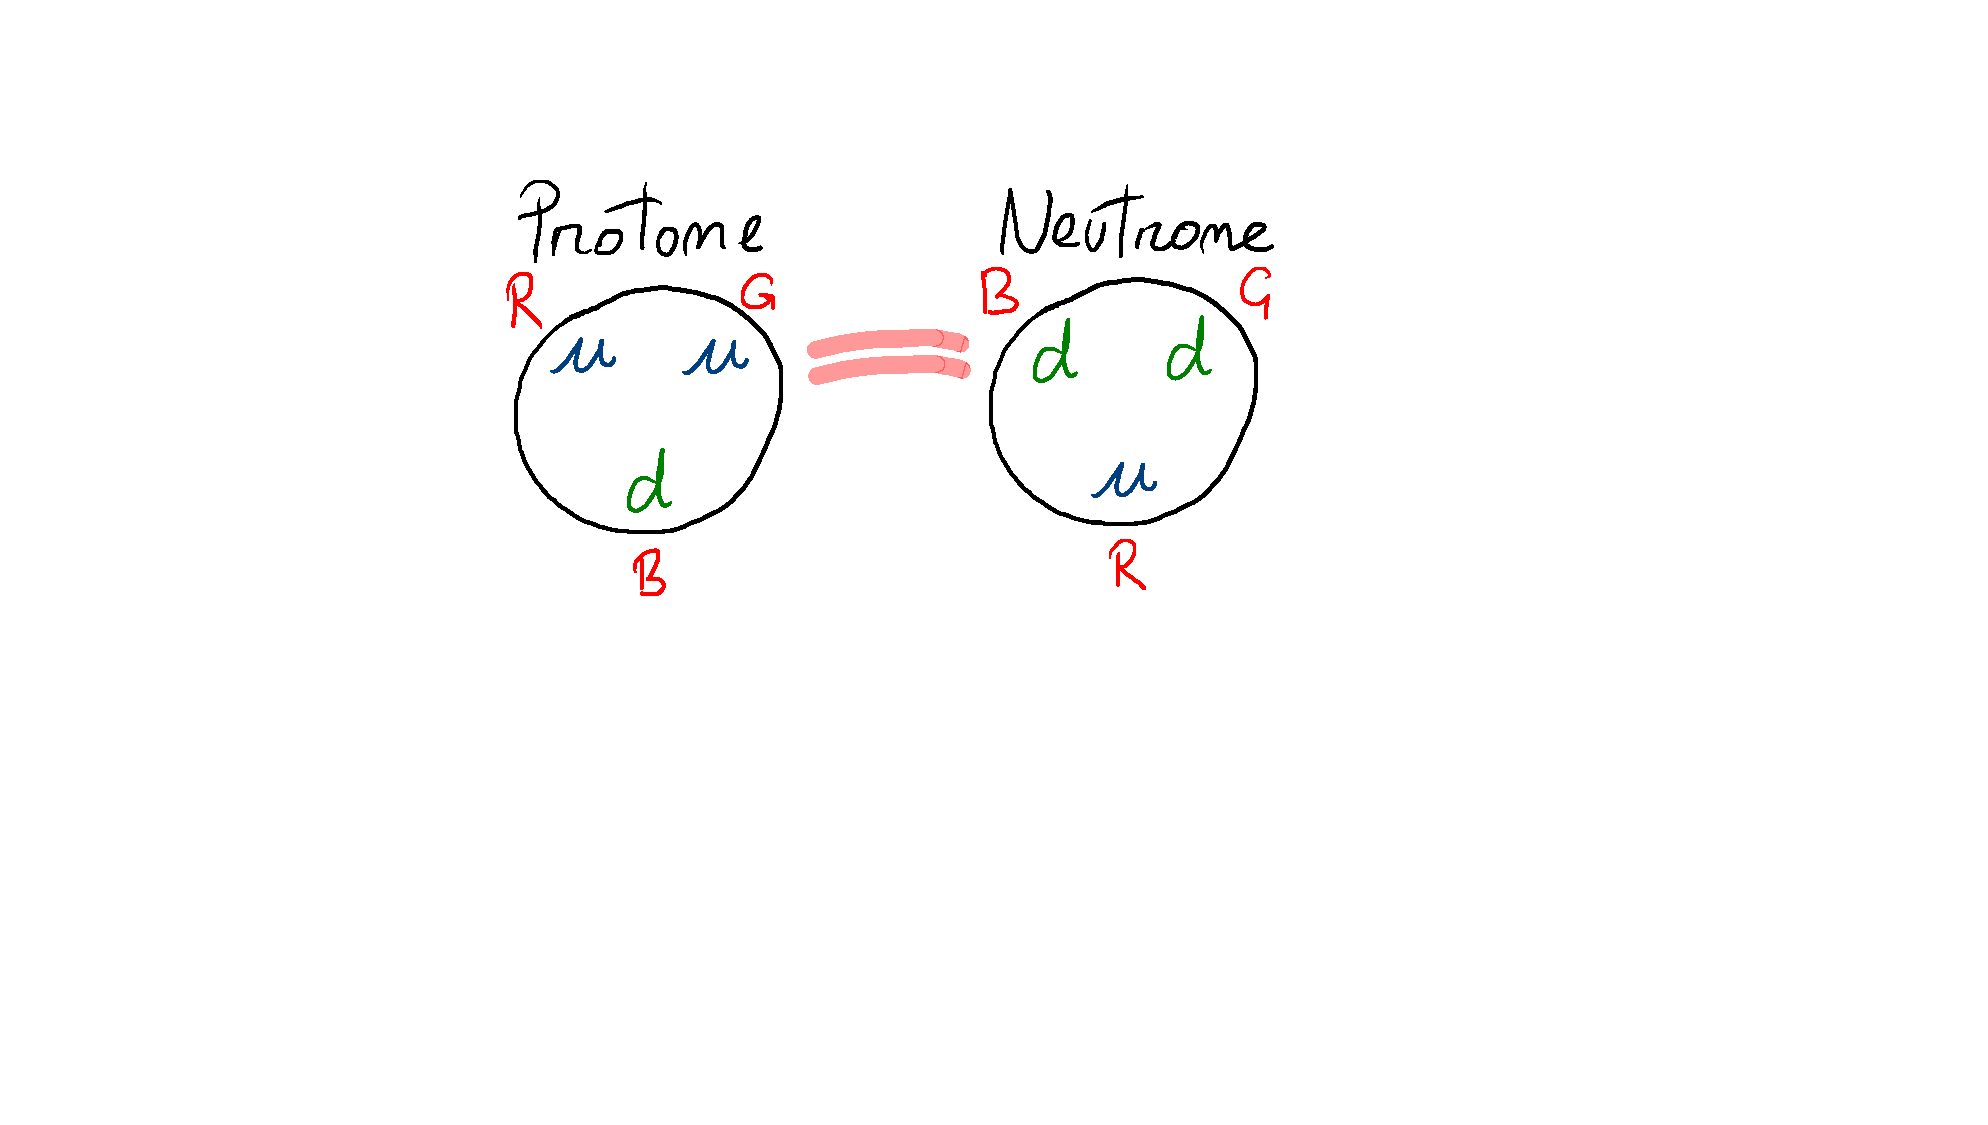
\includegraphics[scale=0.5]{/protone_neutrone_quark}
\caption{CAPTION}
\end{figure}

\paragraph{Carica di colore} I quark hanno anche un secondo tipo di carica: la \emph{carica di colore} che regola l'\emph{interazione forte} tra i quark.
La carica di colore può essere di tre tipi: Red (R), Green (G), Blue (B).
La somma delle tre cariche di colore dei rispettivi quark di un nucleone è nulla
\begin{equation}
R + G + B = 0
\end{equation}
un quark rosso (R) attira un quark verde (G) che attira un quark blu (B), mentre i quark dello stesso colore si respingono.
La teoria fondamentale della QCD esprime come l'interazione nucleare si possa interpretare come la carica di colore residua.

\paragraph{Il potenziale tra nucleoni} è un potenziale di interazione del tipo
\begin{figure}[h]
\centering
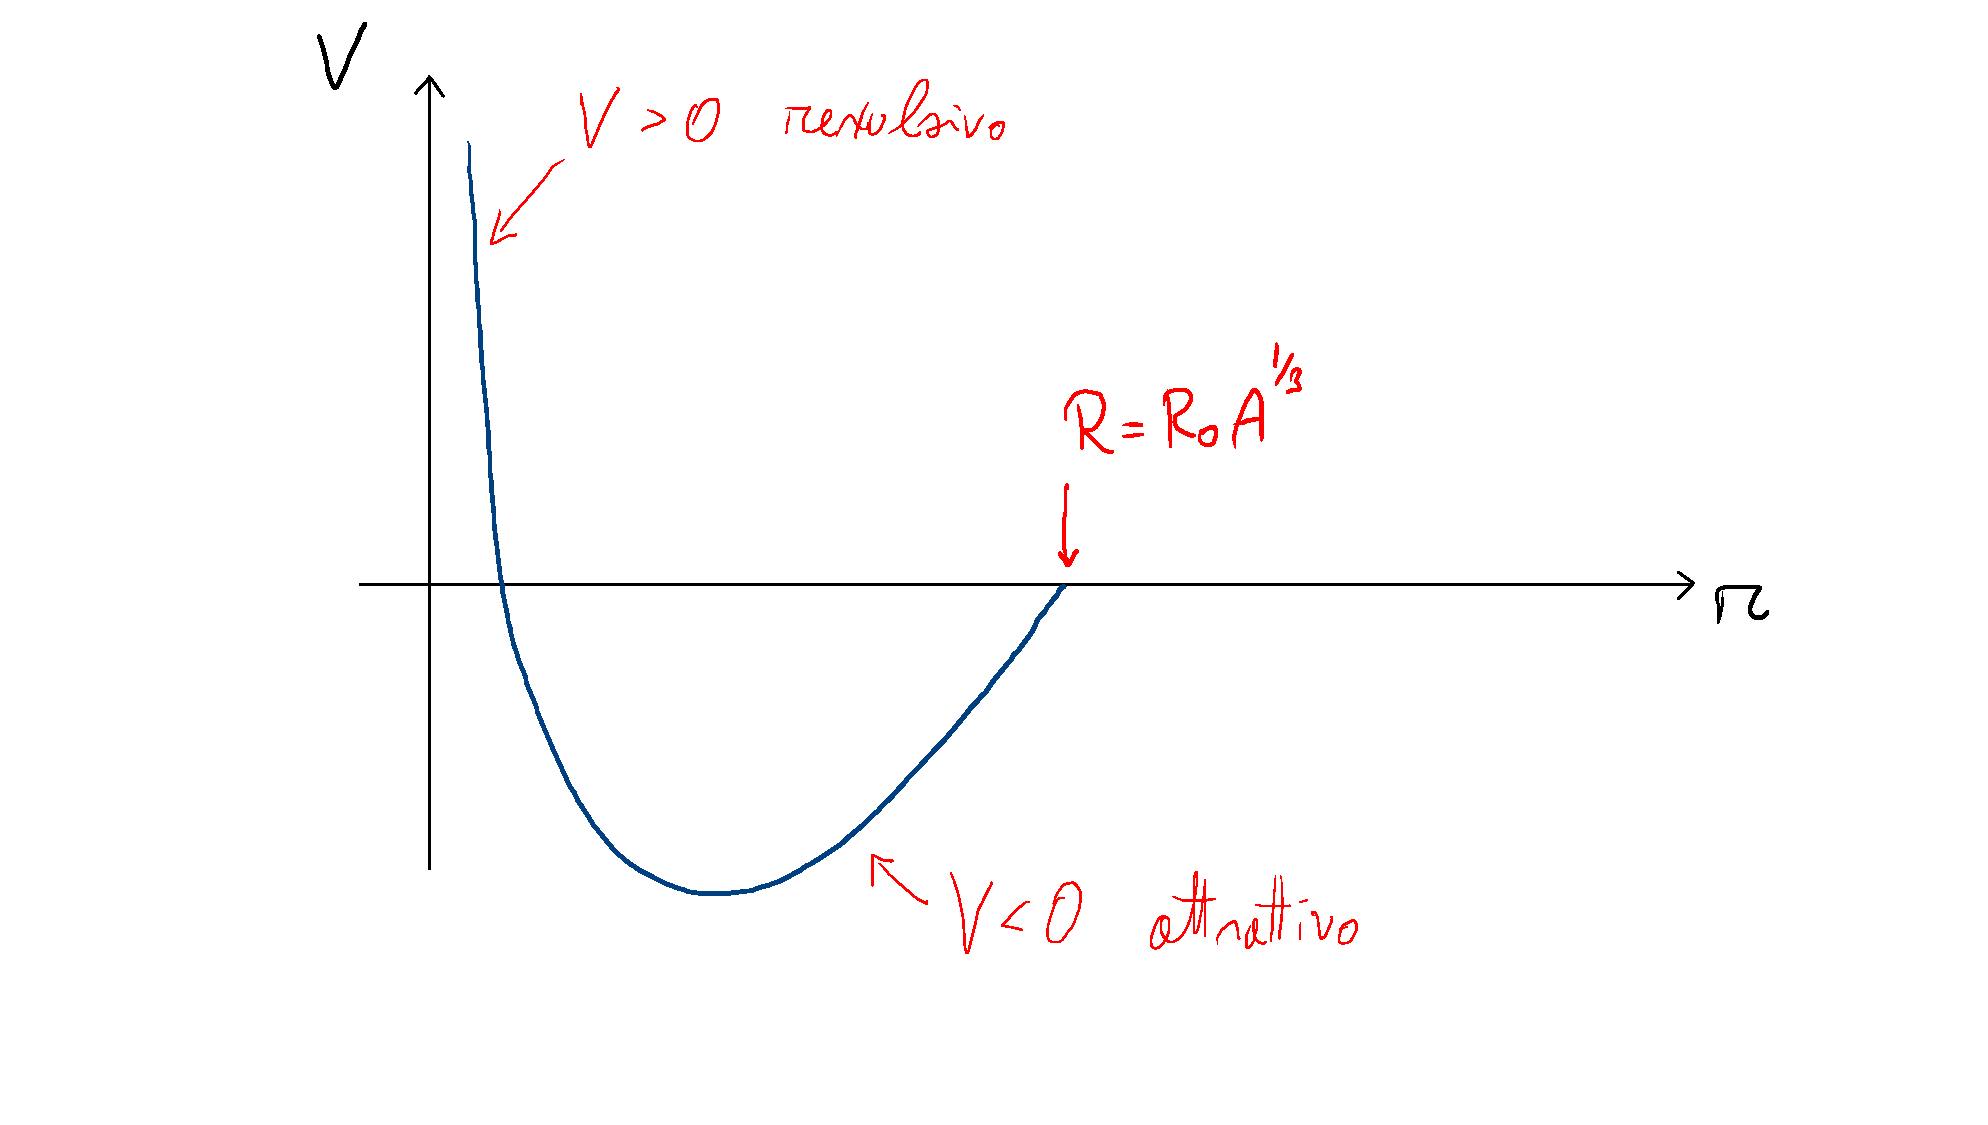
\includegraphics[scale=0.4]{/potenziale_nucleare_1}
\caption{CAPTION}
\end{figure}
Nella prima parte del potenziale si ha che per piccole distanze è \emph{positivo}, ovvero repulsivo, poiché altrimenti i nuclei \underline{privi di dimensione (?)} collasserebbero, ciò è legato al Principio di Esclusione di Pauli, nella seconda parte il potenziale è \emph{attrattivo} ed è ciò che "intrappola" i nucleoni all'interno del nucleo, inoltre oltre alla distanza data da $R = R_0 A^{\frac{1}{3}}$ la forza nucleare è nulla.

\paragraph{Il Deutone} è il nucleo del deuterio, è composto da un protone e un neutrone ed è il più semplice nucleo su cui studiare la forza nucleare.
Del deutone conosciamo l'energia di legame $E_B = \SI{-2.225}{MeV}$ e la distanza tra i nucleoni $R = \SI{2.1}{fm}$ ottenuti sperimentalmente.
Conosciamo inoltre che lo stato legato del deuterio è quello in cui gli spin sono paralleli, dato ottenuto dalla misurazione del momento magnetico, per cui lo spin del deutone è $S = 1$.
\begin{figure}[h]
\centering
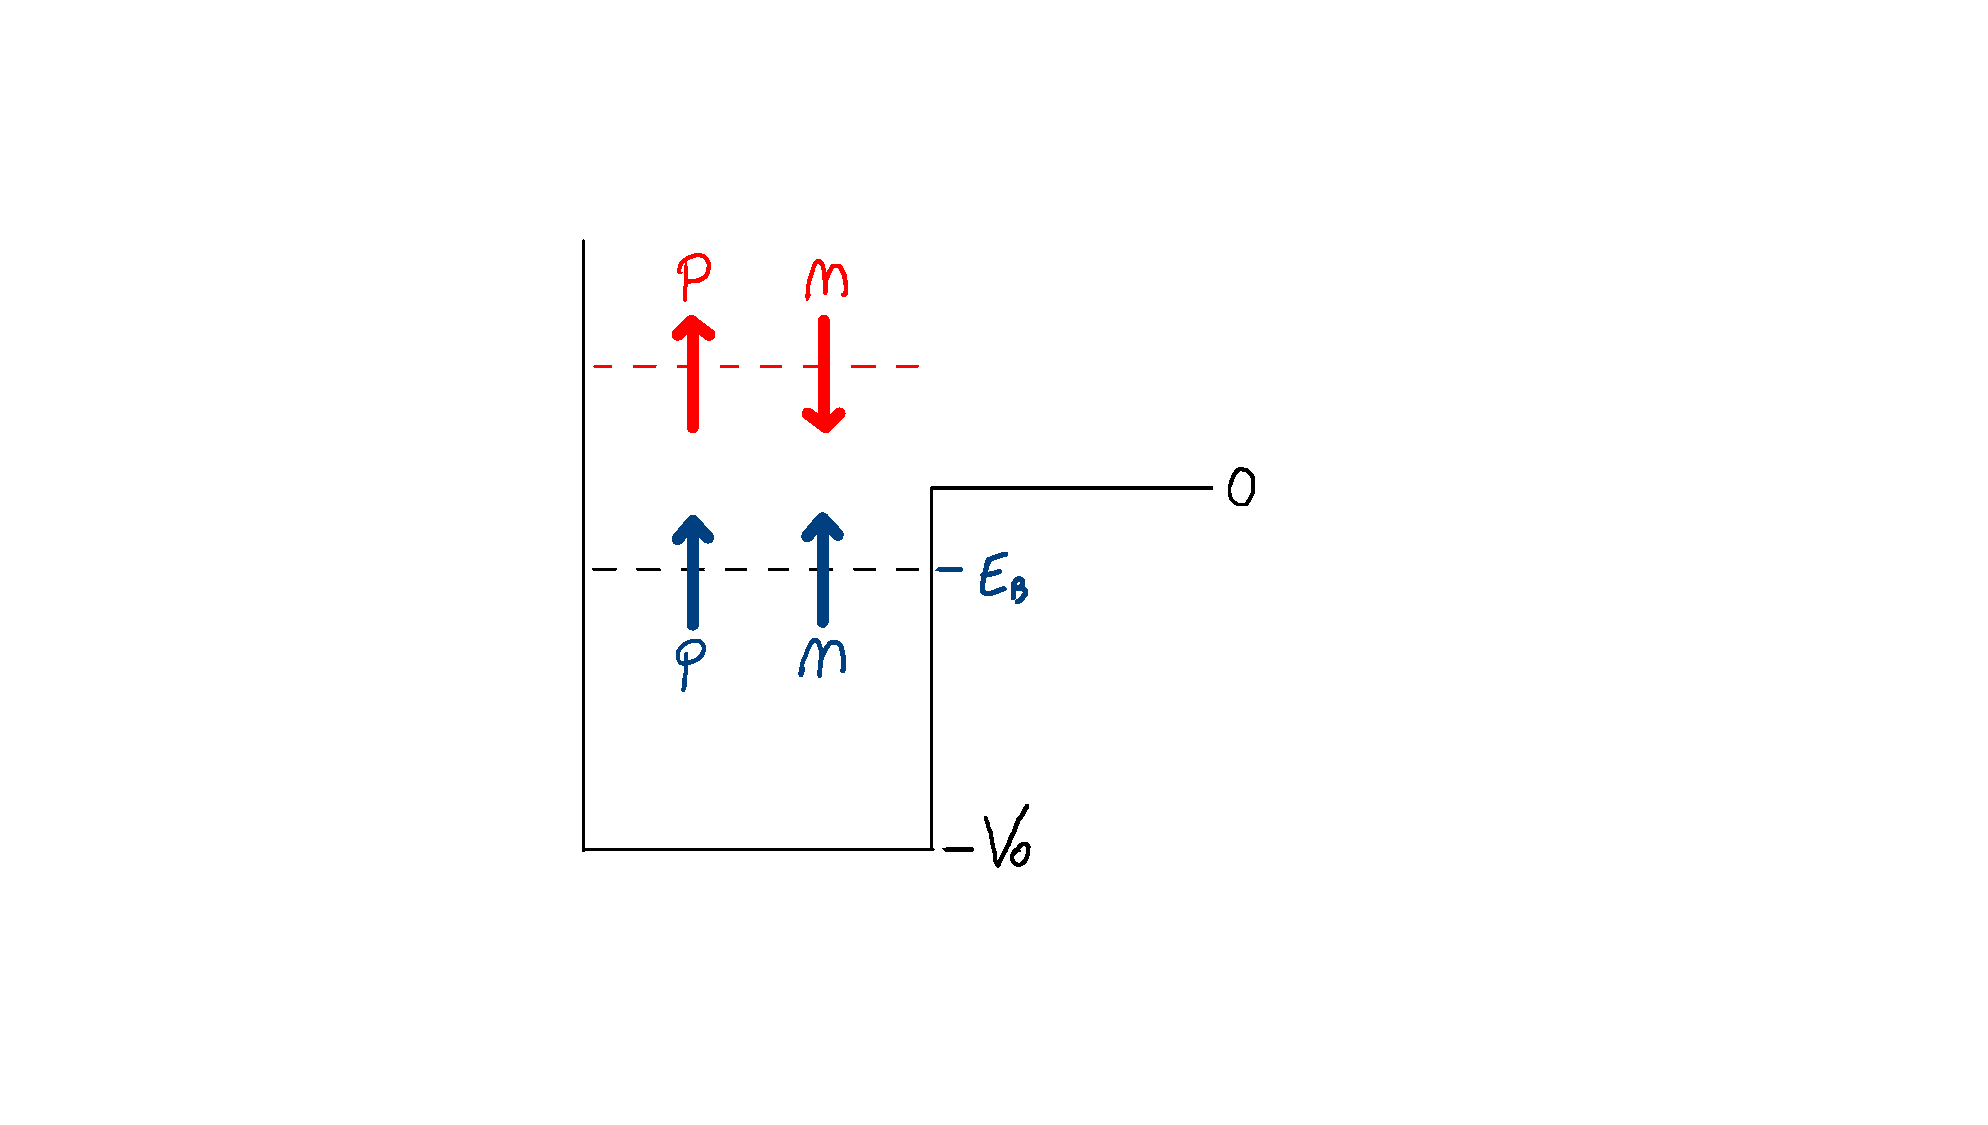
\includegraphics[scale=0.5]{/spin_deutone}
\caption{CAPTION}
\end{figure}
Uno stato con spin anti-parallelo corrisponde ad uno stato non legato, quindi fuori dalla buca di potenziale.
L'interazione nucleare dipende fortemente dallo spin.

Cerco ora il valore della buca di potenziale $V_0$, sommo l'energia cinetica $KE$ con l'energia potenziale $PE$
\begin{equation}
\begin{split}
E & = KE + PE \\
E_B & = KE + V_0
\end{split}
\end{equation}
scrivendo la funzione d'onda trovo il legame con il potenziale $V$
\begin{equation}
\begin{split}
H \psi & = E \psi \\
- \frac{\hbar^2}{2m} \frac{d^2}{dr^2} \psi + V \psi & = E \psi
\end{split}
\end{equation}
Il potenziale di questa buca è
\begin{equation}
V = 
\Bigg\{\begin{array}{l}
V_0 \quad\mbox{zona \Romannum{1}: dentro la buca} \\
0 \quad\mbox{ zona \Romannum{2}: altrove}
\end{array}
\end{equation}
Scrivo l'equazione di Schrodinger nella zona \Romannum{1}, in cui ho $V = V_0$
\begin{equation}
\begin{split}
- \frac{\hbar^2}{2m} \frac{d^2 \psi}{d r^2} + V_0 \psi & = E \psi \\
\frac{d^2 \psi}{d r^2} & = -\frac{2m}{\hbar^2} (E - V_0) \psi \\
\frac{d^2 \psi}{d r^2} & = - K^2 \psi \quad\quad \mbox{con } K^2 = \frac{2m}{\hbar^2} (E - V_0)
\end{split}
\end{equation}
la soluzione ha un andamento oscillatorio ed in generale è
\begin{equation}
\psi(r) = A \sin Kr + B \cos Kr
\end{equation}
calcolo $A$ e $B$ imponendo le condizioni al contorno:
\begin{equation}
\psi (0) = 0 \quad\Rightarrow\quad \psi(0) = A \sin 0 + B \cos 0 = 0 \quad\Rightarrow\quad B=0
\end{equation}
per cui diventa
\begin{equation}
\psi = A \sin K r
\label{psi_1}
\end{equation}
Scrivo l'equazione di Schrodinger nella zona \Romannum{2}, in cui ho $V =0$
\begin{equation}
\begin{split}
\frac{d^2 \psi}{d r^2} & = -\frac{2m}{\hbar^2} E \psi \\
\frac{d^2 \psi}{d r^2} & = L^2 \psi \quad\quad \mbox{con } L^2 = - \frac{2m}{\hbar^2} E
\end{split}
\end{equation}
la soluzione ha un andamento esponenziale ed in generale è
\begin{equation}
\psi(r) = C e^{L r} + D e^{- L r}
\end{equation}
di cui so che deve appartenere allo spazio di Hilbert, per cui la parte $e^{L r}$ non è soluzione in quanto non verifica la condizione $|\psi|^2 < \infty$, per cui diventa
\begin{equation}
\psi(r) = D e^{- L r} 
\label{psi_2}
\end{equation}
Eguagliando le funzioni d'onda \ref{psi_1} e \ref{psi_2} e le loro derivate in corrispondenza della frontiera $r = R$ trovo
\begin{equation}
\Bigg\{\begin{array}{l}
\psi_{\Romannum{1}}(R) = \psi_{\Romannum{2}}(R)\\
\psi_{\Romannum{1}}'(R) = \psi_{\Romannum{2}}'(R)
\end{array}
\quad\Rightarrow\quad 
\Bigg\{\begin{array}{l}
A \sin K R = D e^{ - L R }\\
K A \sin K R = -L D e^{ - L R }
\end{array}
\end{equation}
dividendo una con l'altra le equazioni del sistema trovo la relazione seguente in funzione dei parametri $K$ ed $L$
\begin{equation}
\begin{split}
K & = \sqrt{\frac{2m}{\hbar^2} (E - V_0)} \in \mathbb{R} \\
L & = \sqrt{- \frac{2m}{\hbar^2} E} \in \mathbb{R}
\end{split}
\end{equation}
che quindi diventa
\begin{equation}
\begin{split}
& K \cot K R = - L \\
& \sqrt{\frac{2m}{\hbar^2} (E - V_0)} \cot \Bigl[ R \sqrt{\frac{2m}{\hbar^2} (E - V_0)} \Bigr] = - \sqrt{- \frac{2m}{\hbar^2} E}
\end{split}
\end{equation}
da cui, inserendo i dati sperimentali, 
\begin{equation}
\begin{split}
E & = \SI{-2.225}{MeV} \\
R & = \SI{2.1}{fm}
\end{split}
\end{equation}
e la massa corrisponde alla massa ridotta tra il protone ed il neutrone
\begin{equation}
m = \frac{m_n m_p}{m_n + m_p} \simeq \frac{m_p^2}{2 m_p} = \frac{m_p}{2}
\end{equation}
trovo il valore della buca di potenziale
\begin{equation}
V_0 = \SI{-36}{MeV}
\end{equation}
(non è ben noto come sia davvero possibile risolvere l'equazione del tipo $x \cot a x = b$ ma ok, prendiamo atto del risultato precedente e andiamo avanti).

Risulta quindi che la buca di potenziale del Deutone è profonda $\SI{-36}{MeV}$ di cui solo $\SI{-2.225}{MeV}$ sono di energia potenziale, \emph{di legame}, mentre circa $\SI{-34}{MeV}$ sono di energia cinetica.

Per il ferro $^{56}_{26}Fe$ ad esempio si ha un'energia di legame media di circa $\SI{8}{MeV / nucleone}$, mentre
per il deutone $^{2}_{1}He$ si ha circa $\SI{1.1}{MeV / nucleone}$.

Troviamo tre punti notevoli della funzione d'onda:

\begin{itemize}
\item Quanto vale la funzione d'onda nel punto $r=R$?
In tale punto la funzione vale $\sin K R$ per cui conoscendo i dati trovo
\begin{equation}
\begin{split}
& R = \SI{2.1}{fm} \\
& K = \sqrt{ \frac{2m}{\hbar^2} (E - V_0) } \simeq \SI{0.9}{fm^{-1}} \\
& \sin K R = \sin (0.9 \cdot 2.1) = 0.95
\end{split}
\end{equation}

\item In che punto si ha il valore massimo della funzione d'onda?
\begin{equation}
\begin{split}
& \sin K r = 1 \\
& K r = \frac{\pi}{2} \\
& r = \frac{\pi}{2} \frac{1}{K} \simeq \SI{1.74}{fm}
\end{split}
\end{equation}

\item In che punto la funzione d'onda vale circa $\frac{1}{3}$?
\begin{equation}
\begin{split}
e^{ - L r } & \quad L = \sqrt{\frac{2mE}{\hbar^2}} \to \frac{1}{L} = \SI{4.4}{fm} \\
e^{ - L r } & \rightarrow e^{ \frac{-L}{L}} = e^{ -1 } = 0.37
\end{split}
\end{equation}
\end{itemize}
La funzione d'onda ottenuta evidenzia come sia possible trovare la particella al di fuori della buca di potenziale, a distanze oltre i $\SI{5}{fm}$.











%\include{sections/NUOVOCAPITOLO}

%\include{sections/NUOVOCAPITOLO}

%\include{sections/NUOVOCAPITOLO}


\newpage
%% commento iniziale
%% anche su più righe ma vicine


% ogni file = un capitolo 

\section{Convenzioni LaTex} %inizia il capitolo con "section"
Iniziare a scrivere subito sotto al comando section per dare un senso estetico al codice.
Andare a capo ad ogni "punto", ogni frase inizia una nuova riga di codice.
Lasciando uno spazio bianco (due volte "invio") si ottiene un nuovo inizio paragrafo.

Tipo questo, che non sempre è bello da vedere mentre altre volte è molto utile.
Il concetto è: scrivere il codice il più attaccato possibile ma con maggior leggibilità possibile.

Le equazioni si possono scrivere in vari modi, ma i migliori, per compatibilità tra versioni sono:
\begin{enumerate}
\item equazione nel testo tipo $\cos \alpha = \frac{\pi}{2 \pi}$

\item equazione a capo a centro pagina e su una riga, senza numero di equazione
$$ \frac{d\sigma}{d\Omega}=\frac{b(\theta)}{\sin\theta}\frac{db}{d\theta} $$

\item equazione a capo a centro pagina e su una riga, con numero di equazione 
\begin{equation}
\Delta p_x \Delta x \ge \frac{\hbar}{2}
\end{equation}

\item equazione a capo a centro pagina su più righe, con numero di equazione
\begin{equation}
\begin{split}
\mbox{\underline{Maxwell-Boltzmann}}  \quad\quad  \frac{n_s}{g_s} & = \frac{1}{e^{\alpha + \beta E_s}} \\
\mbox{\underline{Bose-Einstein}}  \quad\quad  \frac{n_s}{g_s} & = \frac{1}{e^{\alpha + \beta E_s} - 1} \\
\mbox{\underline{Fermi-Dirac}}  \quad\quad  \frac{n_s}{g_s} & = \frac{1}{e^{\alpha + \beta E_s} + 1 } 
\end{split}
\end{equation}

\end{enumerate}



\end{document}



